\item If $f(x)$ and $g(x)$ are changed on the region $x \in [0, 4]$, on which region in the $(x, t)-$plane will the solutions of $u_{tt} = 9u_{xx}$ be altered?

%____________________________________________________________________________%
Here, we are given a wave equation on the $x$ boundary $[0, 4]$ and a constant $3^2$.

Here, let us consider our wave equation, $u_{tt} = 9u_{xx}$, where $\sqrt{c} = 3$.

Here, the slope of our characteristic line is $\frac{1}{3}$. If we alter $f(x)$ and $g(x)$, we are changing the range of influence of our equation. For instance, let us pick $x_1 = 1$ for $f(x)$, we would obtain a range of influence such as the following:
%
\begin{center}
  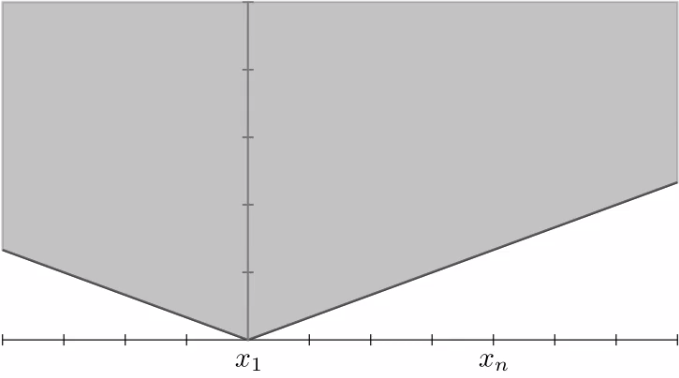
\includegraphics[height=6cm]{2a}
\end{center}

Next, let us consider another point within our boundary, such as $x_n$, let us consider how our graph appears at $f(x_n)$:
%
\begin{center}
  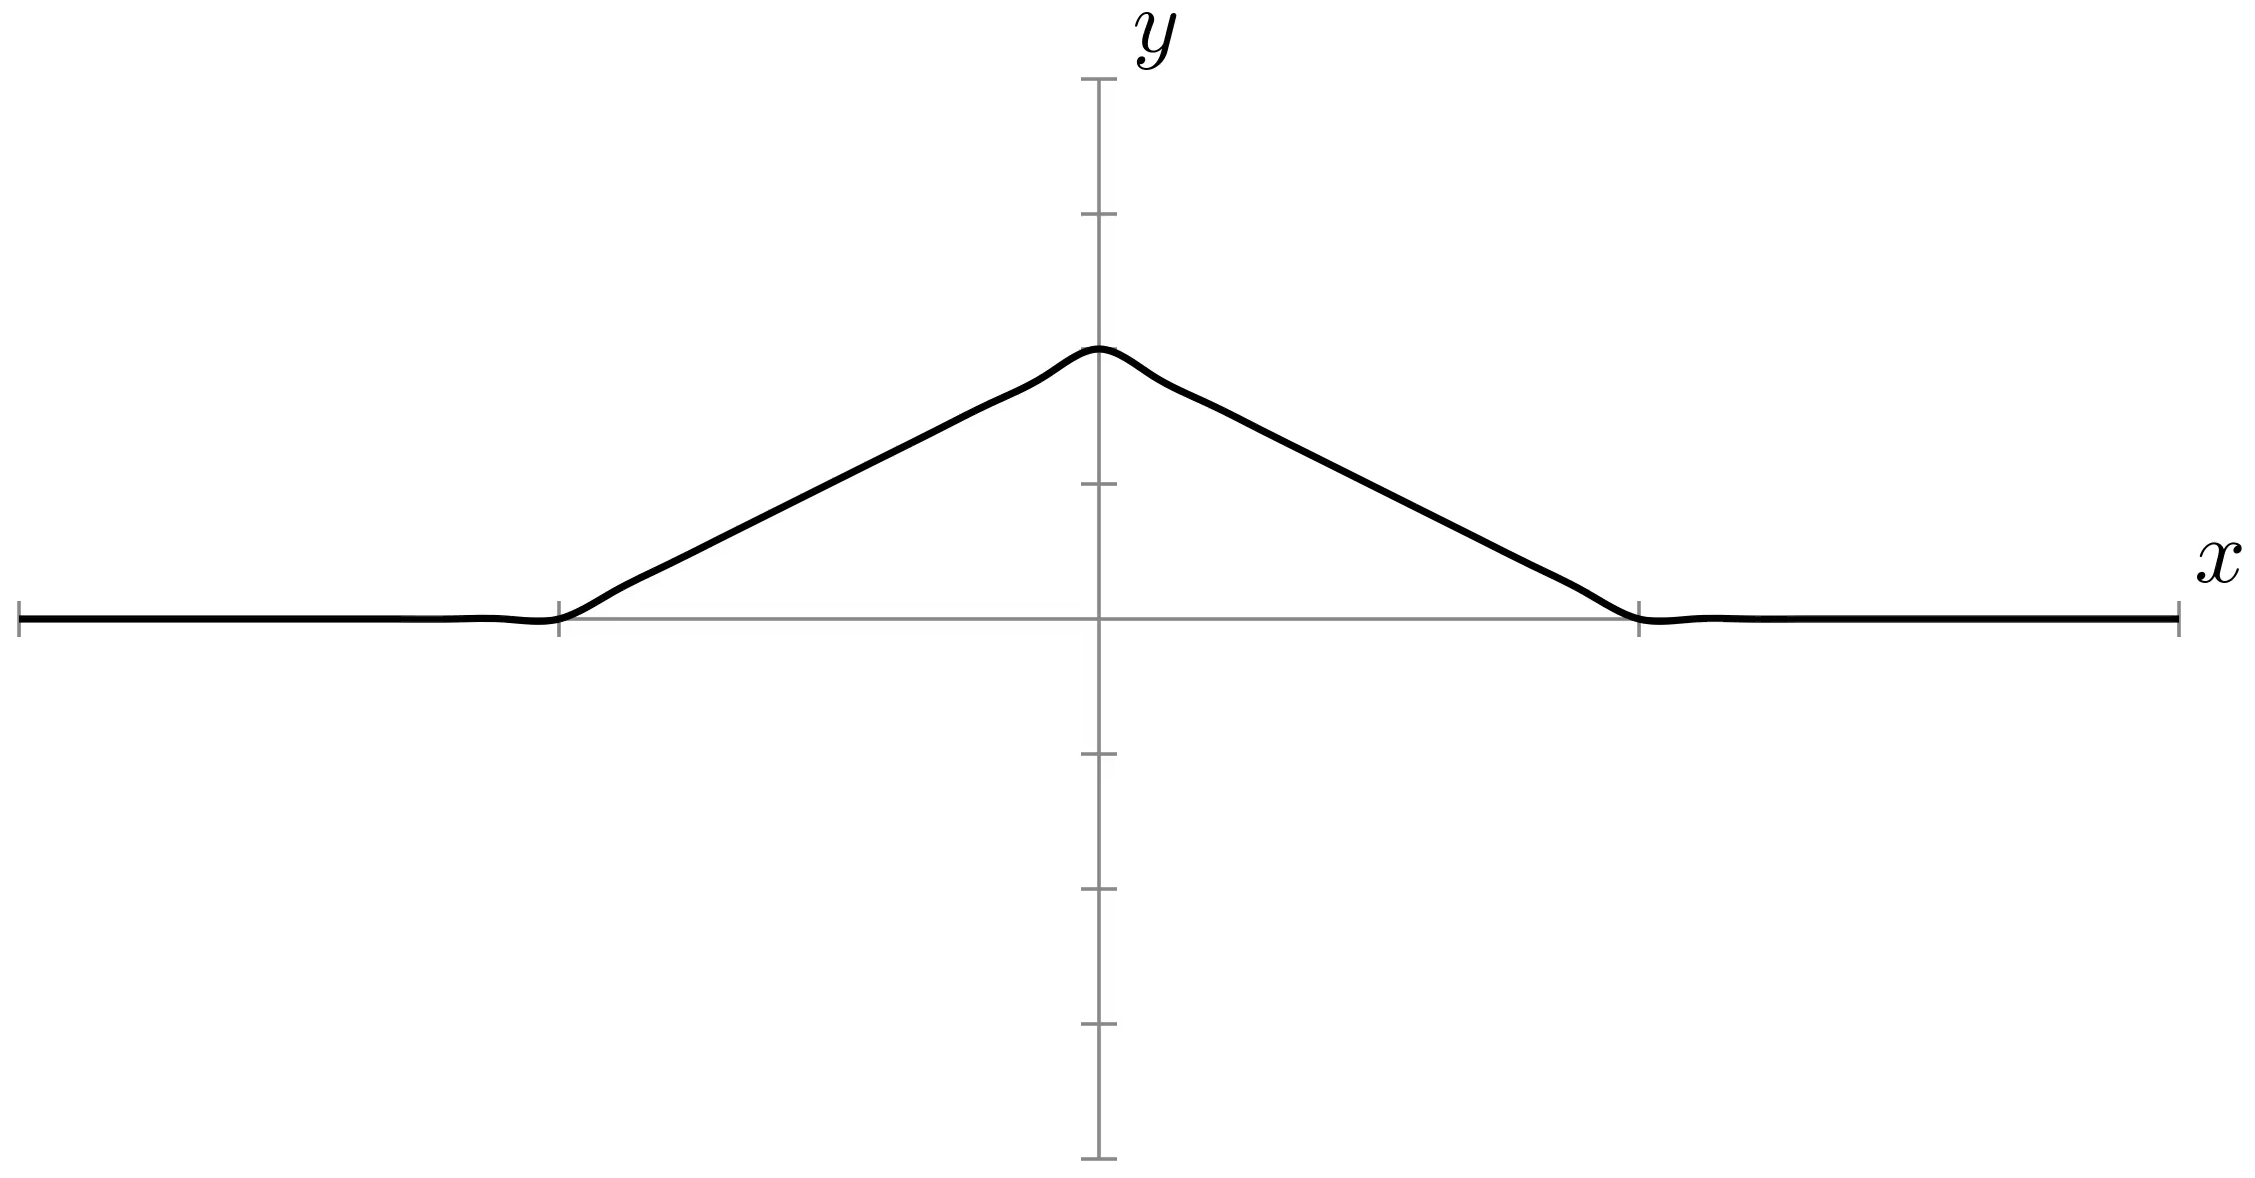
\includegraphics[height=6cm]{2b}
\end{center}

In essence, our range of influence as we tweak $f(x)$ and $g(x)$ lies between the points $x_1$ and $x_n$:
%
\begin{center}
  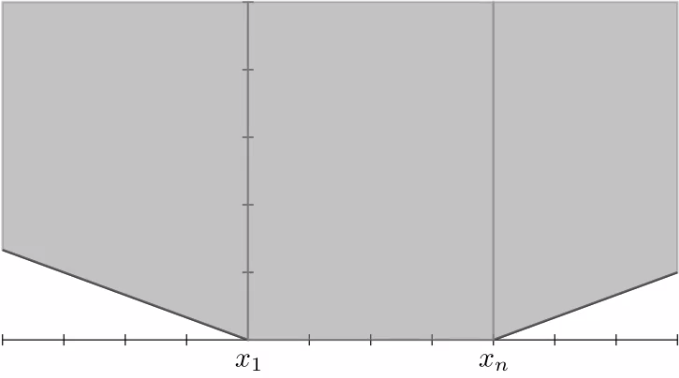
\includegraphics[height=6cm]{2c}
\end{center}
